\chapter{Testing programs}

A software bug is an error in a computer program that causes it to produce an incorrect result or behave in an unintented manner. The term bug was used by Thomas Edison in 1878\footnote{\url{https://en.wikipedia.org/wiki/Software_bug}, possibly \url{http://edison.rutgers.edu/NamesSearch/DocImage.php3?DocId=LB003487}}, but made popular in computer science by Grace Hopper, who found a moth interferring with the electronic circuits of the Harward Mark II electromechanical computer and coined the term \idx{bug} for errors in computer programs. The original bug is shown in Figure~\ref{fig:bug}.
\begin{figure}
  \centering
  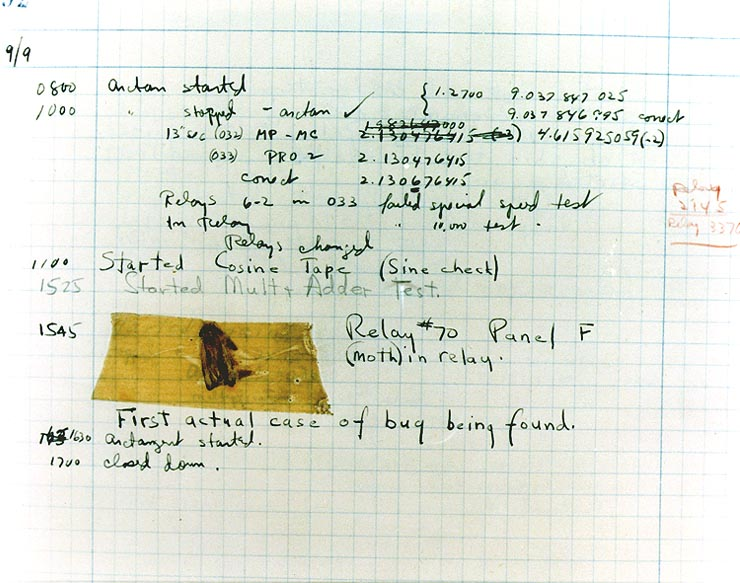
\includegraphics[width=0.45\linewidth]{H96566k}
  \caption{The first computer bug caught by Grace Hopper, U.S. Naval Historical Center Online Library Photograph NH 96566-KN.}
  \label{fig:bug}
\end{figure}

To illustrate basic concepts of software quality consider a hypothetical route planning system. Essential factors of its quality is,
\begin{description}
\item[Functionality:]\idxs{functionality} Does the software compile and run without internal errors. Does it solve the problem, it was intended to solve? E.g., does the route planning software finde a suitable route from point a to b?
\item[Reliability:]\idxs{reliability} Does the software work reliably over time? E.g., does the route planning software work in case of internet dropouts?
\item[Usability:]\idxs{usability} Is the software easy and intuitive to use by humans? E.g., is it easy to enter adresses and alternative routes in the software's interface?
\item[Efficiency:]\idxs{efficiency} How many computer and human resources does the software require? E.g., does it take milliseconds or hours to find a requested route? Can the software run on a mobile platform with limited computer speed and memory?
\item[Maintainability:]\idxs{maintainability} In case of the discovery of new bugs, is it easy to test and correct the software? Is it easy to extend the software with new functionality? E.g., is it easy to update the map with updated roadmaps and new information? Can the system be improved to work both for car drivers and bicyclists? 
\item[Portability:]\idxs{portability} Is it easy to port the software to new systems such as new server architecture and screen sizes? E.g., if the routing software originally was written for IOS devices, will it be easy to port to Android systems?
\end{description}
The above mentioned concepts are ordered based on the requirements of the system. Functionality and reliability ares perhaps the most important concepts, since if the software does not solve the specified problem, then the software designing process has failed. However, many times the problem definition will evolve along with the software development process. But as a bare minimum, the software should run without internal errors and not crash under well defined set of circumstances. Further, it is often the case, that software designed for the general public requires a lot of attention to the usability of the software, since in many cases non-experts are expected to be able to use the software little or no prior training. On the other hand, software used internally in companies will be used by a small number of people, who become experts in using the software, and it is often less important that the software is easy to understand by non-experts. An example is text processing software Microsoft Word versus Gnu Emacs and LaTeX. Word is designed to be used by non-experts for small documents such as letters and notes, and relies heavily on interfacing with the system using click-interaction. On the other hand, Emacs and LaTeX are for experts for longer and professionally typeset documents, and relies heavily on keyboard shortcuts and text-codes for typesetting document entities. 

The purpose of \idx{software testing} is to find bugs. For errors found we engage in \idx{debugging}, which is the process of diagnosing and correcting bugs. Once we have a failed software test, i.e., one that does not find any bugs, then we have strengthened our belief in the software, but it is important to note, that software testing and debugging rarely removes all bugs, and with each correction or change of software, there is a fair chance of introducing new bugs.

In this chapter, we will focus on two approaches to software testing, which emphasizes functionality: \idx[white-box testing]{white-box} and \idx{black-box testing}. An important concept in this context is \idx{unit testing}, where the program is considered in smaller pieces, called units, and for which accompanying programs for testing can be made, which tests these units automatically.

\begin{comment}
  http://www.scientificamerican.com/article/pogue-5-most-embarrassing-software-bugs-in-history/, 5 Most Embarrassing Software Bugs in History

  http://royal.pingdom.com/2009/03/19/10-historical-software-bugs-with-extreme-consequences/

  https://raygun.com/blog/2014/05/10-costly-software-errors-history/

  Mars Climate Observer failure due to unit of measure mixup.

  http://www.computerworld.com/article/2515483/enterprise-applications/epic-failures--11-infamous-software-bugs.html

  http://catless.ncl.ac.uk/Risks/20.59.html#subj1

  https://en.wikipedia.org/wiki/List_of_software_bugs

  December 19, 1991; ISO/IEC 9126, international standard for the evaluation of software quality, replaced by ISO/IEC 25010:2011. Not publically available, \footnote{A review of the ISO/IEC 9126 is given in \url{http://www.sqa.net/iso9126.html}. A brief review of ISO/IEC 25010:2011 is given in }
\end{comment}

%%% Local Variables:
%%% TeX-master: "fsharpNotes"
%%% End:
